% Vorlage für eine Bachelorarbeit - 2012-2013 Timo Bingmann

% Dies ist nur eine Vorlage. Strikte Vorgaben wie die Bachelorarbeit auszusehen
% hat gibt es nicht. Darum können auch alle Teile angepasst werden.

%\documentclass[12pt,a4paper,twoside]{scrartcl}
\documentclass[a4paper,12pt,bibtotoc,titlepage, liststotoc,BCOR7mm,headsepline,pointlessnumbers]{scrbook}

% Diese (und weitere) Eingabedateien sind in UTF-8
\usepackage[utf8]{inputenc}

\usepackage[T1]{fontenc}
\usepackage{times}
\typearea[current]{current}
\usepackage{fancyhdr}
\newenvironment{code}{\begingroup\footnotesize \verbatim}{\endverbatim\endgroup}

\addtokomafont{caption}{\small} % Aktive Auszeichnung von Legenden
\setkomafont{captionlabel}{\sffamily\bfseries}
\bibliographystyle{plain}

% Sprache des Dokuments (für Silbentrennung und mehr)
\usepackage[english,german]{babel}

% Einrückung und Abstand zwischen Paragraphen
\setlength\parskip{\smallskipamount}
\setlength\parindent{0pt}

% Einige Standard-Mathematik Pakete
\usepackage{latexsym,amsmath,amssymb,mathtools,textcomp}

% Unterstützung für Sätze und Definitionen
\usepackage{amsthm}

\newtheorem{Satz}{Satz}[section]
\newtheorem{Definition}[Satz]{Definition}
\newtheorem{Lemma}[Satz]{Lemma}

\numberwithin{equation}{section}

% Unterstützung zum Einbinden von Graphiken
\usepackage{graphicx}

% Pakete die tabular und array verbessern
\usepackage{array,multirow}

% Kleiner enumerate und itemize Umgebungen
\usepackage{enumitem}

\setlist[enumerate]{topsep=0pt}
\setlist[itemize]{topsep=0pt}
\setlist[description]{font=\normalfont,topsep=0pt}

\setlist[enumerate,1]{label=(\roman*)}

% TikZ für Graphiken in LaTeX
\usepackage{tikz}
\usetikzlibrary{calc}

% Hyperref für Hyperlink und Sprungtexte
\usepackage{xcolor}

\usepackage[plainpages=false,pdfpagelabels=false,citecolor=Black, linkcolor=Black]{hyperref} %Verweise werden Links im PDF

% Paket zum Setzen von Algorithmen in Pseudocode mit kleinen Stilanpassungen
\usepackage[ruled,vlined,linesnumbered,norelsize]{algorithm2e}
\DontPrintSemicolon
\def\NlSty#1{\textnormal{\fontsize{8}{10}\selectfont{}#1}}
\SetKwSty{texttt}
\SetCommentSty{emph}
\def\listalgorithmcfname{Algorithmenverzeichnis}
\def\algorithmautorefname{Algorithmus}

\usepackage{Sweave}
\begin{document}
\Sconcordance{concordance:Plot.tex:Plot.Rnw:%
1 73 1 1 0 293 1}


%%%%%%%%%%%%%%%%%%%%%%%%%%%%%%%%%%%%%%%%%%%%%%%%%%%%%%%%%%%%%%%%%%%%%%

\pagestyle{empty} % keine Seitenzahlen
\renewcommand{\thepage}{\roman{page}}

% Titelblatt der Arbeit
\begin{titlepage}

  \begin{center}\large
  \begin{flushleft}
    \quad\includegraphics[height=17mm]{kit_logo_de.pdf} \hfill
     
  \end{flushleft}
    %\includegraphics[height=20mm]{grouplogo-algo-blue.pdf}\quad\null

    \vfill
    \vfill
    \vfill
    \vfill

    Bachelor thesis
    \vspace*{2cm}

    {\bf\huge Title of Thesis  \par}
    % Siehe auch oben die Felder pdftitle={}
    % mit \par am Ende stimmt der Zeilenabstand

    \vfill

    Name of author

    \vspace*{15mm}

    Date: \today 

    \vspace*{40mm}
    \begin{tabular}{rl}
      Supervisors: & Prof. Dr. Peter Sanders \\
      & Dipl. Inform. Zweiter Betreuer \\
    \end{tabular}
    
    \vspace*{10mm}

    %Institut für Theoretische Informatik, Algorithmik \\
    %Fakultät für Informatik \\
    %Karlsruher Institut für Technologie

    \vspace*{10mm}
    % English:
     Institute of Theoretical Informatics, Algorithmics \\
     Department of Informatics \\
     Karlsruhe Institute of Technology

    \vspace*{12mm}
    \vfill
  \end{center}

\end{titlepage}

%%%%%%%%%%%%%%%%%%%%%%%%%%%%%%%%%%%%%%%%%%%%%%%%%%%%%%%%%%%%%%%%%%%%%%
%%%%%%%%%%%%%%%%%%%%%%%%%%%%%%%%%%%%%%%%%%%%%%%%%%%%%%%%%%%%%%%%%%%%%%

%\vspace*{0pt}\vfill
\ 
\newpage
\clearpage

\section*{Abstract}
In this thesis we augment the existing Hypergraph Partitioner KaHyPar with an evolutionary framework with the goal to improve the 
solution quality.
\addcontentsline{toc}{chapter}{Abstract}
\selectlanguage{english}
% German and English Abstract
\vfill\vfill\vfill
\ 
\newpage
\clearpage
\ 
\newpage
\clearpage

%%%%%%%%%%%%%%%%%%%%%%%%%%%%%%%%%%%%%%%%%%%%%%%%%%%%%%%%%%%%%%%%%%%%%%
\section*{Acknowledgments}

I'd like to thank Timo for the supply of Club-Mate
\vfill\vfill\vfill
Hiermit versichere ich, dass ich diese Arbeit selbständig verfasst und keine anderen, als die angegebenen Quellen und Hilfsmittel benutzt, die wörtlich oder inhaltlich übernommenen Stellen als solche kenntlich gemacht und die Satzung des Karlsruher Instituts für Technologie zur Sicherung guter wissenschaftlicher Praxis in der jeweils gültigen Fassung beachtet habe.

\bigskip
\vspace*{1cm}
\noindent
Ort, den Datum

\clearpage

%%%%%%%%%%%%%%%%%%%%%%%%%%%%%%%%%%%%%%%%%%%%%%%%%%%%%%%%%%%%%%%%%%%%%%
\tableofcontents
\clearpage
%%%%%%%%%%%%%%%%%%%%%%%%%%%%%%%%%%%%%%%%%%%%%%%%%%%%%%%%%%%%%%%%%%%%%%
\clearpage
%%%%%%%%%%%%%%%%%%%%%%%%%%%%%%%%%%%%%%%%%%%%%%%%%%%%%%%%%%%%%%%%%%%%%%
\mainmatter
\pagestyle{plain}
\chapter{Introduction}
\pagestyle{headings}
\section{Motivation}
Hypergraph Partitioning is a highly complex field of study. The Motivation behind this work is to add an evolutionary
framework to the existing Hypergraph partitioner KaHyPar in order to improve the cuts of the Hypergraph.
\section{Contribution}
\section{Structure of Thesis}
%%%%%%%%%%%%%%%%%%%%%%%%%%%%%%%%%%%%%%%%%%%%%%%%%%%%%%%%%%%%%%%%%%%%%%
\chapter{Fundamentals}
\section{General Definitions}
A Hypergraph $H = (V, E, c, w)$ is defined as a set of verticies $V$ a set of hyperedges $E$ where each edge may contain an arbitrarily large subset of $V$.
$c: V \rightarrow  \mathbb R_{\ge 0}$ is a function applying a weight to each Vertex and $w: E \rightarrow  \mathbb R_{\ge 0}$ applying a weight to each hyperedge. 
Two verticies $u, v$ are adjacent if $\exists e \in E | u, v \in e$ and a vertex $u$ is incident to a hyperedge $e$ if $ u \in e$. The size $|e|$ of an Hyperedge $e$ is the number of verticies contained in $e$. A k-way partition of a Hypergraph $H$ is a partition of $V$ into k disjoint blocks $V_1, .. V_k$. $part: V \rightarrow [0, k-1]$ is a function referencing the corresponding block of a k-way partition to a vertex $u$. 
A k-way partition is balanced when the weight of each block $V_i | 1 \le i \le k, \sum_{v_i \in V_i} c(v_i) \le (1 + \epsilon) \lceil \frac{\sum_{v \in V} c(v)}{k} \rceil $  for a balance constraint $\epsilon$.
A valid solution is a balanced k-way partition. An invalid solution is a partition where either the balance criterion is not met, or $H$ has been partitioned for a different value for k.
A Hyperedge $e$ is a cut edge $cut(e)$ if $\exists u,v \in e | part(u) \neq part(v)$. The connectivity of a Hyperedge $e$ is $\lambda(e)$ = $\sum_{i=0}^{k-1} \delta(e,i) | \delta(e, i) = 
     \begin{cases}
       \text{1} &\exists v \in e\text{ }part(v)=i\\
       \text{0} &\text{else}\\
     \end{cases}$ 

The set cut edges in H is defined as
$cut(E) := \{e \in E | cut(e) \}$.
The multiset connectivity edges in H is defined as
$conn(E) := \{a(e) \in E | cut(e) \} |a(e) := \lambda(e)$
The cut metric $cut(H) := \sum_{e \in E} 
\begin{cases}
       \text{w(e)} & \text{e is cut edge}\\
       \text{0} &\text{else}\\
     \end{cases}$  and gives the value of cuts.
The connectivity metric $(\lambda -1)(H) := \begin{cases}
       \text{$\lambda(e)*w(e)$} & \text{e is cut edge}\\
       \text{0} &\text{else}\\
     \end{cases}$
Both metrics can be used to measure the quality of a solution. Throughout this thesis the solution quality is referenced. The metrics are interchangeable in this regard.
An Individual $I$ is a valid solution for the k-way partition problem of $H$.
An individual eligible for further operations is considered $alive$.
%TODO ominus = sym set diff
The difference of two individuals $I_1, I_2$ is $diff(I_1, I_2) := cut(I_1) \ominus cut(I_2)$
The connectivity difference of two individuals $I_1, I_2$ is $strongdiff(I_1, I_2) := conn(I_1) \ominus conn(I_2)$
A population $P$ is a collection of Individuals.

\begin{figure}[t!] 
    \vspace*{-.25cm}
  \centering
   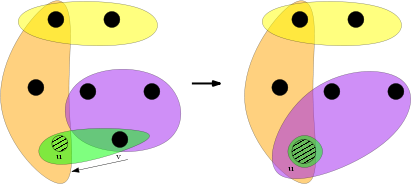
\includegraphics[width=.8\textwidth]{Ipe/img.png} %TODO PDF
  \caption{An example of a contraction. Note that the Hyperedges of the reduced node $v$ are rearranged to contain $u$.}\label{fig:img.png}
    \vspace*{-.5cm}
\end{figure}


%Hypergraph := (H;V;E;C)
%Node contraction := 
%Node uncontraction := 
%Net :=
%cut :=
%onnectivity :=
%quality :=
%p%opulation :=
%individual :=
%solution := 
%mbalance:= 
\chapter{Related Work}
The Hypergraph Partitioner KaHyPar uses a multilevel approach for partition. The original Hypergraph $H$ is coarsened by repeadeatly contracting nodes $u,v$ until either no more contractions are possible due to the size of the contracted nodes or that the minimum amount of nodes required to be in the coarsened Hypergraph $H_c$ has been reached. During each step of the coarsening only one pair of nodes $u, v$ is contracted. Nodes for contraction are chosen to contract multiple high weight edges to emphasize that $u,v$ should most likely share the same partition. 
%TODO explain node selection for coarsening 
On $H_c$ partitioning algorithm is chosen to generate an initial partitioning. Contracted nodes acquire the partition of their corresponding representing node.  Afterwards to contraction operations will be reverted and 
during each step of the uncoarsening phase local search algorithms are used to improve the current connectivity of $H$. The local search is based on the principle of
Fiduccia-Mattheysis algorithm where operations of decreasing quality are considered, but only executed if the sum of operations results in a net gain.
\newline
\begin{figure}[t!] 
    \vspace*{-.25cm}
  \centering
   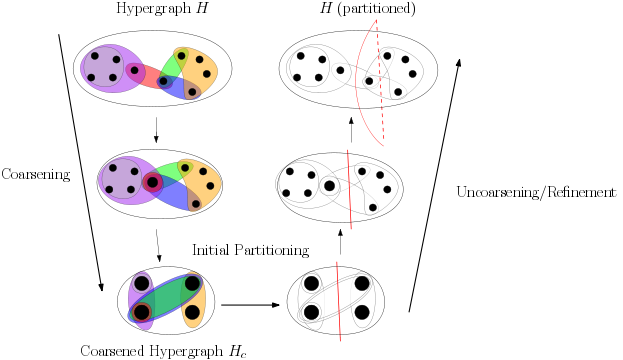
\includegraphics[width=.8\textwidth]{Ipe/iteration.png}
  \caption{An example of an iteration. Coarsening, Initial Partitioning and Refinement}\label{fig:img.png} %TODO u nicht gestrichelt; pünktchen
    \vspace*{-.5cm}
\end{figure}

The memetic Graph Partitioner KaHiP uses evolutionary actions to increase solution quality and is the main inspiration for the operations implemented in KaHyParE.
%KaHyPar
%KaHiP 
%edge-frequency
%%%%%%%%%%%%%%%%%%%%%%%%%%%%%%%%%%%%%%%%%%%%%%%%%%%%%%%%%%%%%%%%%%%%%%
%TODO only one individual is generated per iteration
%TODO explain evolutionary algorithms, or at least show that this is one
\chapter{KaHyParE}
\section{Overview}
The objective of the algorithm is to optimize solution quality of a k-way partition of $H$ within bounded time. During this time
the algorithm will operate on already existing solutions in order to generate improved solutions. Most operators introduced in this 
thesis are using the multilevel approach of KaHyPar as black box, with some alterations towards the general procedure.  
\section{Population}
The algorithm will produce multiple individuals, which are inserted and removed from the population. At any given time only a finite amount of
individuals are $alive$ which is the maximum population size. Furhter individuals have to compete for a place in the population. 
The population size is an important parameter, as a small value limits the solution scope and a high value limits convergence.
We use KaHyPar to fill the initial population.
in order to select a proper population size for the runtime, we dynamically allocate 15\% of the runtime to create and fill the initial population.
\section{Diversity}
By measuring the difference between two individuals we can gain some knowledge over their internal structure and similarities.
using the edges rather than the verticies for difference ensures that only elements relevant for the solution quality are considered
for difference and perturbations of the partition blocks are not influencing the difference. As such we can consider the diversity of
the population as the difference of the current individuals. Therefore a low diversity is a population where the individuals are 
in close proximity considering the solution space or convergent. A high diversity means that the individuals are spread throughout a 
larger portion of the solution space.  
\section{Selection Strategies}
For an evolutionary algorithm we attempt to generate new, improved solutions by using existing solutions. A logical conclusion is that good individuals probably will generate solutions
close to the original individual and as such good. We select our individuals using tournament selection. By first selecting two random individuals and using the one with the better solution quality we can extract one individual while ensuring that better solutions are more likely to be used by the algorithm. For operators requiring two seperate Individuals we can simply redo this step. In the unlikely case that the two selected individuals are the same we instead use the worse individual from the second tournament selection. 
\section{Combine operations}
\subsection{Basic Combine}
The basic combine uses two parent partitions $P_1$ $P_2$ in order to create a child individual $C$. This is achieved by only allowing contractions of nodes $u, v$ when these nodes are not placed in different partitions in either parent. Afterwards we do not perform an initial partitioning, instead we consider the coarsened Hypergraph and see which of the parents gives the better objective on said graph. 
Since the contraction condition is rather strong and we do not need to do an initial partitioning, we can remove the coarsening limit $s$ used by KaHyPar
to allow for more contractions. The uncoarsening and application of local search algorithms which guarantee to atleast maintain solution quality in combination with using the better partition of the two parents ensures that the child solution is at least as good as the best parent solution. It is imporant to note that the combine operation is more powerful the more diverse the parent individuals are, since similar parents are essentially just a vcycle. This will be important in the replacement strategy which will insert the child into the population and is the reason why the selection strategy is avoiding using the same individual. 
\subsection{Cross Combine}

\subsection{Edge Frequency Multicombine}
We also introduce a multi-combine operator, capable of combining multiple individuals $I_1.. I_n, n \le |P|$ into a new child individual. By analyzing whether an edge $e$ is a cut edge in $I_1 ..I_n$ we can calculate the edge frequency of $e$ by $f(e) := \sum_{i=1}^n cut(e,I_i)$. We use the best $n = \sqrt{|P|}$ individuals from $P$ for determining edge frequency. As such, edges with a high frequency are more likely to be cut edges in equally good solutions. Therefore we penalize contractions of nodes incident to a high frequency edge during the multilevel partition approach by using this formula $\frac{1}{(w(u)w(v))^{1.2}}*e^{-\gamma*f(e)}$ to disincentivize early contractions of nodes in edges of high probability. Since these contractions are most likely not improving the quality and will make other, perhaps more favorable contractions invalid. Unlike the other combine operators edge frequency does not set any of the input partitions $I_i$ as current partition of $H$ during the iteration. The only step that differentiates this operator from a regular iteration using KaHyPar is that the rating function during the coarsening is adapted by the penality formula above. It is necessary that an initial partitioning is generated for the coarsened Hypergraph.
%\subsection{Basic Combine + Edge Frequency Information}
\section{Mutation operations}
Mutations are performed on randomly chosen individuals instead of tournament selection.
\subsection{VCycle}
A Vcycle is an iteration in the regular KaHyPar procedure with the difference that $H$ is already partitioned. During the coarsening nodes $u,v$ may only be contracted if $part(u) = part(v)$. Since the Graph is already partitioned there is no need for initial partitioning. The main benefit comes from the refinement during the uncoarsening. This operation takes one individual $I$ and the result is a similar individual $I_c$. Due to the fact that neither refinement nor coarsening worsen the quality of the solution the quality of $I_c$ will also not be worse than $I$. This is a weak mutation and the difference of $I$ and $I_c$ are small. This operation will also cause convergence, as multiple applications of a vcycle will eventually no longer be able to generate improvement and are unable to escape the local optima due to the fact that worse solutions can not be generated.   
\subsection{VCycle + New Initial Partitioning}
Similar to a vcycle we can coarsen $H$ with a set partition, but if the partition is dropped after the coarsening, and a new initial partitioning is performed we have an operation generating a more pertubed solution, while applying the information of the original partition during the coarsening. This operation also takes one individual $I$ and produces an offspring $I_c$. Since the partition is
dropped the algorithm used to generate a new partition might produce a worse solution as before. Therefore this operator can create worse solutions. This operation explores more solution space than regular vcycles.  
\subsection{Stable Nets}
Opposed to edge frequeny where edges of high probability of being in the cut are penalized because these edges are most likely being in the cut regardless, stable net removal attempts to broaden the solution scope by forcefully removing these edges out of the cut. Again the $\sqrt{|P|}$ best individuals are analyzed, regarding edges most frequent in these solutions. These edges are then attempted to be forced into the block with the smallest amount of nodes in order to keep the balance criterion met. Forcefully moved nodes may not be reassigned through another stable net. These solutions have most likely siginficantly worse quality. Due to the nature of our selection strategy these solutions are very unlikely to be used in any combine operator. In order to keep these solutions competitive we also perform a vcycle after removing the stable nets. 
\section{Replacement Strategies}
Regardless of the operator, the generated individual $I_c$ has to be inserted into the population in order to be used in upcoming iterations. 
The naive approach is to remove the worst element from the population and insert $I_c$ in its place, with the intention to ensure a vast majority of the best generated solutions. The consequence is that the population is rapidly converging towards a local optima and only covering a small amount of the solution space. Another approach is to replace the element used in the operator. This strategy was originally used for mutations, as the theory behind evolutionary algorithms is to pertubate an existing solution. Instead trying to merge two objectives for the replacement strategy, quality and diversity, there is a compromise strategy which replaces the most similar element to $I_c$ that is also worse than $I_c$ in terms of quality. The most natural approach towards this problem is to use the difference metric to the corresponding quality metric. As a result incompetitive solutions are removed entirely and the replaced element is in relatively close neighborhood towards the newly generated solution which ensures more granular steps through the solution space. 
%.....
%%%%%%%%%%%%%%%%%%%%%%%%%%%%%%%%%%%%%%%%%%%%%%%%%%%%%%%%%%%%%%%%%%%%%%
\chapter{Experimental Evaluation}
We evaluate our algorithm on two Hypergraph sets. One time for different $k = \{2,4,8,16,32,64,128\}$ and 174 Hypergraph Instances, repeating
each run 5 times with different seeds and a algorithm runtime of 8 hours. This is referenced as benchmark subset. The other evaluation is a
selection of 25 Hypergraphs using only one $k = 32$ and a runtime of 2 hours. This is referenced as tuning subset. 
As such our datasets contain multiple tuples of $(H, k, s, t, \lambda)$ where $H$ is the instance, $s$ the seed, $t$ the required time and $\lambda$ the solution quality. An Instance $I$ is the subset of $(H, k, s, t, \lambda)$ where $H$ and $k$ are fixed.
The main interest is the best solution over time compared to other partitioning algorithms. Unfortunately most graphs vary drastically in solution quality and time required to perform one iteration. We solve the time differences by not using the measured time, but rather the normalized time. 
In order to do so we choose one of the partitioning algorithms $p$ as baseline and determine the average duration $t_I$ of an iteration for each $I$. Afterwards for each $I$ the normalized time $t_n$ is calculated by $t_n = \frac{t}{t_I}$. We then generate a list for each instance containing $(s, t_n, \lambda)$ sorted by $t_n$. Now we generate the averaged improvements for $I$. For each seed $s$ a value $a_s$ is reserved and the list is read in. When $(s, t_n, \lambda)$ is better than the reserved value for $s$ the average over all $a_s$ 
is the new value appended to the averaged improvements with($(avg(a), t_n)$. Similarly we now reserve a value $a_I$ for each Instance of averaged improvements and calculate a new list of general improvements by calculating the geometric mean over all $a_I$. 
\begin{figure}[t!] 
    \vspace*{-.25cm}
  \centering
   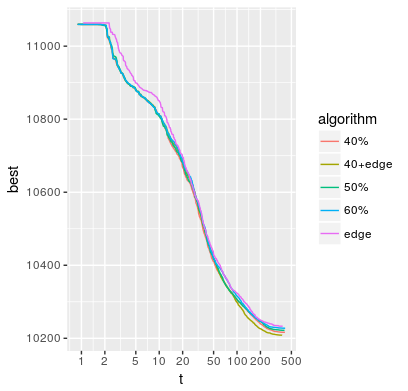
\includegraphics[width=.8\textwidth]{img/edge frequency.png}
   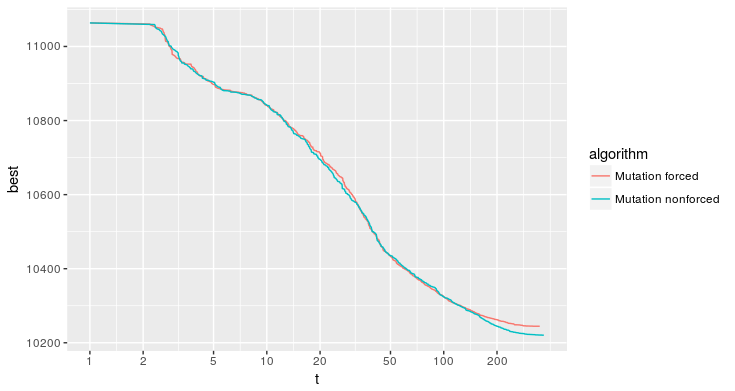
\includegraphics[width=.8\textwidth]{img/forced_nonforced_mutation.png}

  \caption{Caption}
    \vspace*{-.5cm}
\end{figure}
\begin{figure}[t!] 
    \vspace*{-.25cm}
  \centering

   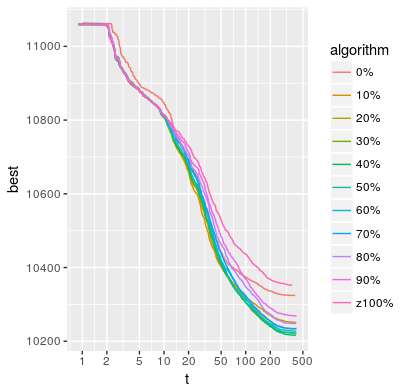
\includegraphics[width=.8\textwidth]{img/newip_tuning.png}
   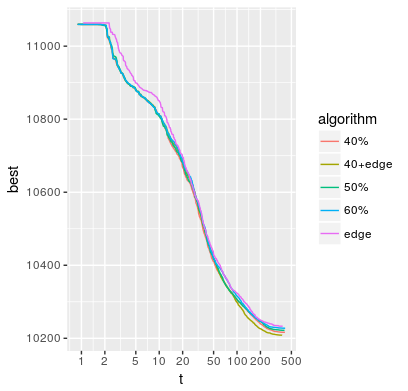
\includegraphics[width=.8\textwidth]{img/edge frequency.png}

  \caption{Caption}
    \vspace*{-.5cm}
\end{figure}
\begin{figure}[t!] 
    \vspace*{-.25cm}
  \centering

   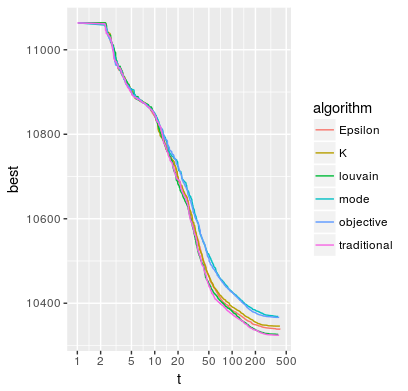
\includegraphics[width=.8\textwidth]{img/cross combines.png}
  \caption{Caption}
    \vspace*{-.5cm}
\end{figure}
\section{Implementation}
\section{Experimental Setup}
\subsection{Environment}
\subsection{Tuning Parameters}
\subsection{Instances}
\section{Your Experiment Headline}
%%%%%%%%%%%%%%%%%%%%%%%%%%%%%%%%%%%%%%%%%%%%%%%%%%%%%%%%%%%%%%%%%%%%%%
\chapter{Discussion}
\section{Conclusion}
\section{Future Work}
Vcycles härter
Kreativere auswahlstrategie

\clearpage
\begin{appendix}
\chapter{Implementation Details}
\section{Software}
% Data Structures etc..
\section{Hardware}
\end{appendix}
%%%%%%%%%%%%%%%%%%%%%%%%%%%%%%%%%%%%%%%%%%%%%%%%%%%%%%%%%%%%%%%%%%%%%%
\bibliographystyle{gerplain}
\bibliography{literatur}
\end{document}
